Enterprises such as Visual Solutions use firewalls to enforce Internet Protocol access policies at the edge of their networks. These policies relate to who is allowed to access which resources. The firewall is often implemented using 5-tuple rules (source and destination IP address, source and destination ports, and transport protocol). Typically, firewalls were developed to handle client-server protocols such as web browsing, email, and file transfer\cite{johnston_taking_2013}. Peer-to-peer communication systems are bigger challenges to firewalls, and since \gls{wrtc} is designed to work peer-to-peer, this introduces some problems. This is why \gls{ice} was developed, to make firewall traversal easier. But enterprise communication software usually has a client-server architecture. To communicate with entities outside the enterprise network, it is common to use a \gls{sbc}. Current \gls{sbc}s won't work well with \gls{wrtc}. This is because WebRTC is such a new technology, that SBC vendors haven't had time to address this issue yet. This raises some problems:

\begin{itemize}
\item{How can the enterprise firewall detect and apply policy to \gls{wrtc} flows?}
\end{itemize}

\section{Session border controllers}

\begin{figure}[here]
\centerline{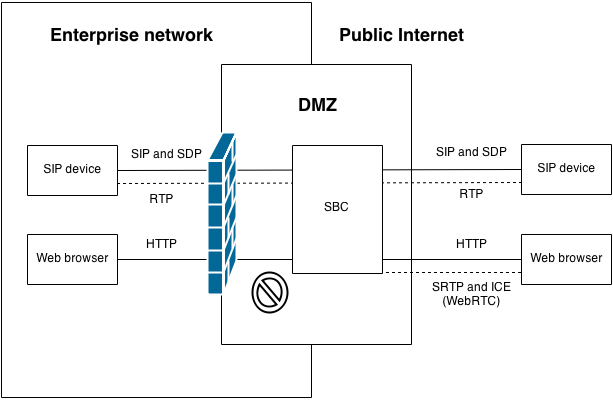
\includegraphics[scale=0.5]{sbcpolicy.png}}
\caption{The SBC opens firewall to allow for enterprise communication, but WebRTC media path is blocked.}
\label{fig:sbc-policy}
\end{figure}

A \gls{sbc} is a device that is essentially an application layer firewall with a signaling and media application layer gateway built in. The \gls{sbc} is usually connected in an enterprise demilitarized zone (DMZ) as a trusted enterprise network element. It blocks all unauthorized signaling and media flows, and provides a point of policy enforcement as shown in Figure \ref{fig:sbc-policy}. As specified by IETF\cite{sbc} a \gls{sbc} should support \gls{sip}, \gls{rtp}, and \gls{srtp}. By parsing \gls{sip} messages, the \gls{sbc} is able to discover the transport addresses (5-tuple) to be used for the media session. The \gls{sbc} opens a filter rule permitting the \gls{rtp} traffic, and the \gls{rtp} media session is able to traverse the firewall. Since \gls{sbc}s are widely deployed it makes sense to reuse them for \gls{wrtc}. The \gls{sbc} should either be upgraded to support \gls{wrtc}, or we should opt for another way of detecting \gls{wrtc} flows.

\section{WebRTC firewall traversal}
If upgrading the \gls{sbc} is non-trivial, we should find other ways for detecting an incoming \gls{wrtc} session. I am not able to do experiments on a SBC, but I will evaluate some suggestions from a paper on WebRTC in an enterprise\cite{johnston_taking_2013}:

\subsection{ICE}
There is a standard type of signaling protocol used for establishing media flows as part of \gls{wrtc}. It is built into the \gls{ice} protocol used for traversing firewalls. Before any media flows, \gls{ice} is run between two WebRTC clients. This could be used to detect an \gls{ice} exchange starting up across the enterprise border. This could then be used to distinguish a \gls{wrtc} media flow across the border, allowing policy to be applied\cite{johnston_taking_2013}. This would work if the SBC is configured to understand STUN and TURN protocols.

\subsection{SRTP}
Another approach might be to use SRTP key negotiation along with \gls{dtls} to authenticate the media flow. For example, since SRTP-DTLS is used for key management, a gateway could act as a man-in-the-middle an hence validate the public key in the fingerprint. A self-signed key from the browser could be stored in an enterprise key server. This could allow the gateway to authenticate the browser inside the enterprise network and apply appropriate policy\cite{johnston_taking_2013}. This means we have to add another component outside our enterprise firewall that authenticates the media flows. This method is in my opinion unnecessary complex.

\subsection{Media relay}
Another approach would be to require a media relay to be used for \gls{wrtc} media sessions crossing the enterprise border. There is a standard protocol for this relay, known as \gls{turn}. The enterprise firewall would be configured to block non-relayed \gls{wrtc} media flows. The enterprise would then deploy a \gls{turn} server in the \gls{dmz}, and permit media flows that go through this server\cite{johnston_taking_2013}. I believe this is a good approach. By forcing the use of relaying the media through a TURN server, the SBC knows that traffic from the TURN server should be allowed to cross the enterprise firewall as seen in Figure \ref{fig:sbc-turn}.

\begin{figure}[here]
\centerline{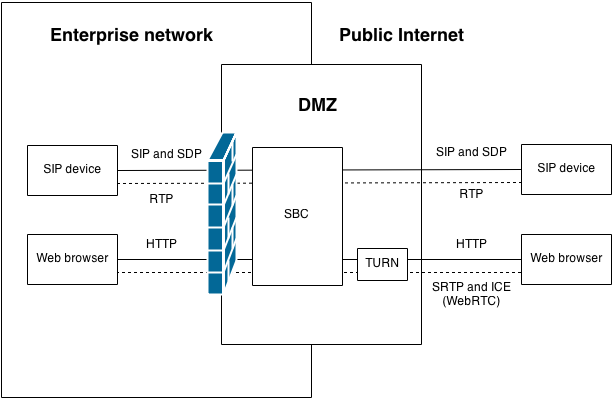
\includegraphics[scale=0.5]{sbcpolicy-wTURN.png}}
\caption{DMZ with SBC and TURN server to allow for both enterprise communication and WebRTC media flows.}
\label{fig:sbc-turn}
\end{figure}

\newpage
\section{Summary}
Doing communication crossing enterprise networks is difficult. It might not be trivial to upgrade current SBC implementations, therefore I evaluated alternative ways of detecting \gls{wrtc} traffic for applying policy to the media flows. A good solution is to configure the SBC/firewall to accept incoming traffic from a TURN server and block everything else, WebRTC media flows would then be relayed through the TURN server.